\chapter{暗物质、轴子和偏振量子通道}
\label{chap:15}

\begin{chapteropening}
暗物质和轻场新物理很少直接给出一张“新粒子图像”。它们更常出现在偏振角、到达时间、相关函数、透镜放大率和像位置的微小偏离里。轴子和轴子样粒子通过 \(aF\tilde F\) 耦合旋转线偏振或在外磁场中与光子转换；超轻暗物质可让这种旋转随时间振荡；黑洞超辐射可在 Kerr 黑洞附近堆积轻玻色云；冷暗物质小晕则通过透镜扰动改变多像系统。QCD axion 的基础、现代 axion cosmology、CAST helioscope、CMB cosmic birefringence、EHT 轴子云搜索和强透镜子结构测量给出了这些信号的主要观测入口 \citep{1977PhRvL..38.1440P,1978PhRvL..40..223W,1978PhRvL..40..279W,1983PhRvL..51.1415S,2016PhR...643....1M,2017NatPh..13..584C,1990PhRvD..41.1231C,1999PhRvL..83.1506L,2020PhRvL.125v1301M,2022NatRP...4..452K,2020PhRvL.124f1102C,2022NatAs...6..592C,1998MNRAS.295..587M,2002ApJ...572...25D}。
\end{chapteropening}

\section{轴子场怎样进入光子的偏振和强度}

这一章的基本态度是先把“新物理”翻译成观测量，再问普通天体物理和仪器能不能模仿它。对轴子和轴子样粒子来说，最常见的两个入口很直接：一个是偏振角被旋转，另一个是外磁场中轴子和光子相互转换，改变某个偏振态或能段的强度。二者都来自同一个相互作用项。

低能有效理论中，轴子样场 \(a\) 与电磁场的相互作用写成
\begin{equation}
  \mathcal L_{a\gamma}
  =
  -\frac{1}{4}g_{a\gamma}aF_{\mu\nu}\tilde F^{\mu\nu}
  =
  g_{a\gamma}a\,{\bf E}\cdot{\bf B}.
  \label{eq:ch15-axion-lagrangian}
\end{equation}
\begin{formulaexplain}[公式 (15.1) 解读]
\(\mathcal L_{a\gamma}\) 是轴子-光子耦合项，\(g_{a\gamma}\) 是耦合强度，\(a\) 是轴子样场，\(F_{\mu\nu}\) 和 \(\tilde F^{\mu\nu}\) 是电磁张量及其对偶。写成 \({\bf E}\cdot{\bf B}\) 后可以看出：这个相互作用只在偏振和磁场方向相关时显现。
\end{formulaexplain}
\(g_{a\gamma}\) 的单位是 \({\rm energy}^{-1}\)，天体和实验文献常用 \({\rm GeV^{-1}}\)。\(F_{\mu\nu}\) 是电磁张量，\(\tilde F^{\mu\nu}\) 是对偶张量；第二个等号把耦合写成 \({\bf E}\cdot{\bf B}\)，只有电场和磁场的相对取向带有手征信息时才起作用。QCD axion 还满足近似质量-衰变常数关系
\begin{equation}
  m_a \simeq
  5.7\,\mu{\rm eV}
  \left(\frac{10^{12}\,{\rm GeV}}{f_a}\right),
  \label{eq:ch15-qcd-axion-mass}
\end{equation}
\begin{formulaexplain}[公式 (15.2) 解读]
\(m_a\) 是 QCD axion 质量，\(f_a\) 是 PQ 对称破缺尺度。尺度越高，轴子越轻；这条关系把 QCD axion 限制在参数图上的一条窄带附近。
\end{formulaexplain}
其中 \(f_a\) 是 PQ 对称破缺尺度。ALP 不必满足这条关系，\(m_a\) 和 \(g_{a\gamma}\) 可以近似独立，因此图上常把 QCD axion band 和更宽的 ALP 参数空间分开 \citep{2016PhR...643....1M,2014JHEP...06..037D}。

外磁场中，轴子和与 \(B_\perp\) 平行的光子偏振态混合。弱混合、均匀磁场、吸收可忽略时，
\begin{equation}
  P_{a\to\gamma}
  \simeq
  \left(\frac{g_{a\gamma}B_\perp L}{2}\right)^2
  \mathrm{sinc}^2\!\left(\frac{qL}{2}\right),
  \qquad
  q\simeq \frac{|m_a^2-m_\gamma^2|}{2E}.
  \label{eq:ch15-axion-conversion}
\end{equation}
\begin{formulaexplain}[公式 (15.3) 解读]
\(P_{a\to\gamma}\) 是轴子转成光子的概率，\(B_\perp\) 是横向磁场，\(L\) 是相干长度，\(q\) 是轴子和光子动量失配。前面的平方项给强度，\(\mathrm{sinc}^2\) 项说明相位失配会破坏相干累积。
\end{formulaexplain}
\(B_\perp\) 是垂直于传播方向的磁场，\(L\) 是相干路径长度，\(E\) 是粒子能量，\(m_\gamma\) 是等离子体中光子的有效质量。\(qL\ll1\) 时振幅沿路径相干相加，概率按 \(L^2\) 增长；\(qL\gtrsim\pi\) 后，相位失配让不同路径段相互抵消。CAST 使用 \(9\,{\rm T}\)、\(9.26\,{\rm m}\) 的 LHC 退役偶极磁体寻找太阳 axion 转换成 X 射线；2013-2015 真空管数据给出 \(g_{a\gamma}<0.66\times10^{-10}\,{\rm GeV^{-1}}\) 的 95\% C.L. 限制，适用于 \(m_a\lesssim0.02\,{\rm eV}\) 的相干低质量区 \citep{2017NatPh..13..584C}。

\begin{figure}[tbp]
\centering
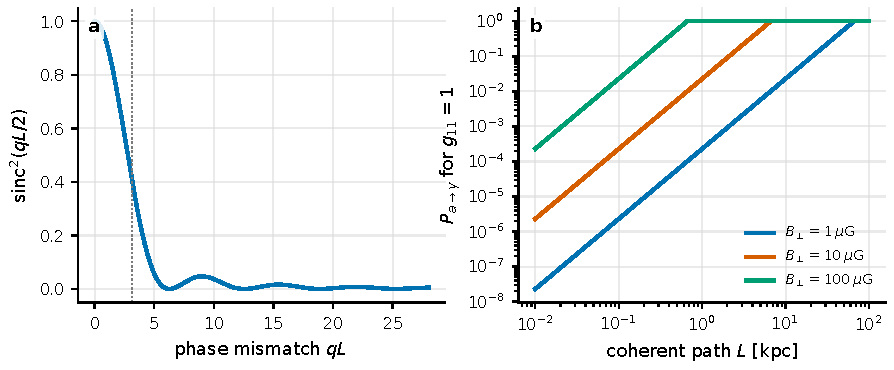
\includegraphics[width=0.94\linewidth]{figures/generated/chapter_15/ch15_axion_conversion.pdf}
\caption{轴子-光子转换由强度和相位共同控制。左图显示 \(\mathrm{sinc}^2(qL/2)\) 的相干因子；当 \(qL\) 接近 \(\pi\) 后，路径不同部分的转换振幅开始抵消。右图给出星际尺度的相干极限数量级，采用 \(g_{11}=g_{a\gamma}/10^{-11}{\rm GeV^{-1}}=1\)；在 \(\mu{\rm G}\) 磁场和 kpc 路径中，单段转换概率通常远小于 1。}
\label{fig:ch15-axion-conversion}
\end{figure}

同一个耦合也会让线偏振角旋转。若光子从发射点 \(e\) 到观测者 \(o\) 穿过缓慢变化的轴子背景，几何光学近似给出
\begin{equation}
  \Delta\psi
  =
  \frac{1}{2}g_{a\gamma}\,[a(t_o,{\bf x}_o)-a(t_e,{\bf x}_e)] .
  \label{eq:ch15-axion-rotation}
\end{equation}
\begin{formulaexplain}[公式 (15.4) 解读]
\(\Delta\psi\) 是线偏振角旋转，括号内是观测端和发射端轴子场的差。它不含 \(\lambda^2\)，因此和 Faraday 旋转最重要的区别是近似无波长依赖。
\end{formulaexplain}
这条旋转与波长无关，和第 \ref{chap:14} 章的 Faraday 旋转 \(\psi=\psi_0+{\rm RM}\lambda^2\) 不同。若轴子构成本地超轻暗物质，
\begin{equation}
  a(t,{\bf x})
  \simeq
  a_0\cos(m_at+\varphi),
  \qquad
  a_0=\frac{\sqrt{2\rho_a}}{m_a}.
  \label{eq:ch15-axion-dm-field}
\end{equation}
\begin{formulaexplain}[公式 (15.5) 解读]
\(a(t,{\bf x})\) 是经典振荡轴子场，\(a_0\) 是振幅，\(\rho_a\) 是轴子暗物质能量密度。质量越小，在同样能量密度下场振幅越大，偏振旋转的时间变化也越慢。
\end{formulaexplain}
\(\rho_a\) 是局部暗物质能量密度，银河系常用 \(0.3\,{\rm GeV\,cm^{-3}}\) 作数量级。振荡周期和相干时间为
\begin{equation}
  T_a
  =
  \frac{2\pi\hbar}{m_ac^2}
  \simeq
  47.9\,{\rm d}
  \left(\frac{10^{-21}\,{\rm eV}}{m_a}\right),
  \qquad
  t_{\rm coh}\sim \frac{T_a}{v^2},
  \label{eq:ch15-axion-timescales}
\end{equation}
\begin{formulaexplain}[公式 (15.6) 解读]
\(T_a\) 是轴子场振荡周期，\(t_{\rm coh}\) 是相干时间，\(v\) 是暗物质速度弥散。超轻质量对应长周期；速度弥散很小，所以同一频率相位可保持许多周期。
\end{formulaexplain}
其中 \(v\sim10^{-3}c\) 是银河系 halo 速度弥散。\(m_a=10^{-21}\,{\rm eV}\) 时，偏振角可在几十天周期上振荡，而相干时间可到 \(10^5\) 年量级。CMB axion dark matter 搜索利用今天本地场的共同振荡和最后散射面处的 washout 效应；Fedderke、Graham 和 Rajendran 指出，普通静态 cosmic birefringence 搜索并不等价于这种快速振荡信号 \citep{2019PhRvD.100a5040F,2021ARA&A..59..247H}。

\begin{figure}[tbp]
\centering
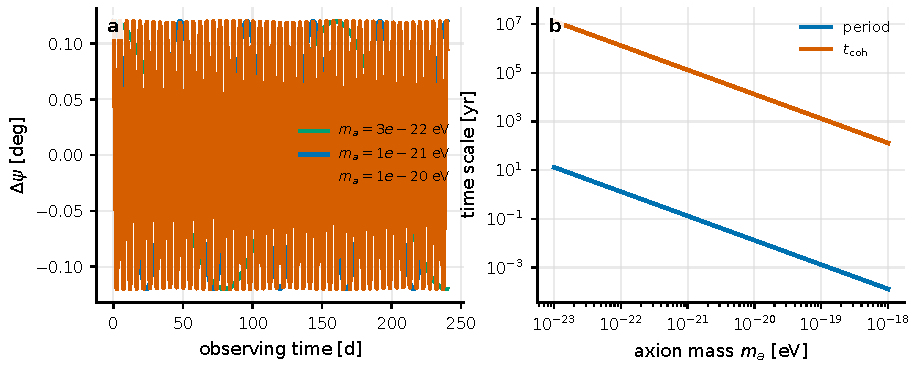
\includegraphics[width=0.94\linewidth]{figures/generated/chapter_15/ch15_axion_polarization_oscillation.pdf}
\caption{超轻暗物质把偏振旋转变成时间序列。左图画出三个轴子质量对应的 \(\Delta\psi(t)\)；质量越大，振荡越快。右图把 \(m_a\) 转换成周期 \(T_a\) 和相干时间 \(t_{\rm coh}\sim T_a/v^2\)，其中 \(v=10^{-3}c\)。}
\label{fig:ch15-axion-oscillation}
\end{figure}

\section{CMB 双折射为什么首先是角标定问题}

CMB 是寻找全局偏振旋转的诱人对象：最后散射面很远，天空覆盖大，统计量可以压到很小。但它也把一个简单问题变成最尖锐的系统误差问题。宇宙本身把偏振转过 \(\beta\)，和探测器偏振角整体错标 \(\alpha\)，在 CMB 谱里几乎长得一样。因而这一节的核心不是先宣布一个非零 \(\beta\)，而是看它怎样与角标定、银河尘埃和偏振泄漏分开。

线偏振 Stokes 参数 \(Q\) 和 \(U\) 旋转角 \(\beta\) 后，
\begin{equation}
  Q\pm iU \rightarrow e^{\pm2i\beta}(Q\pm iU).
  \label{eq:ch15-qu-rotation}
\end{equation}
\begin{formulaexplain}[公式 (15.7) 解读]
\(Q\) 和 \(U\) 是线偏振 Stokes 参数，\(\beta\) 是整体偏振旋转角。指数里的 \(2\beta\) 来自线偏振的自旋 2 性质，因此小角度误差会把 \(E\) 模和 \(B\) 模互相泄漏。
\end{formulaexplain}
在球谐空间中，这会把 \(E\) 模和 \(B\) 模混合。若最后散射面本征 \(EB\) 很小，观测到的 parity-odd 谱近似为
\begin{equation}
  C_\ell^{EB,{\rm obs}}
  =
  \frac{1}{2}\sin(4\beta)
  \left(C_\ell^{EE}-C_\ell^{BB}\right),
  \qquad
  C_\ell^{TB,{\rm obs}}
  =
  \sin(2\beta)C_\ell^{TE}.
  \label{eq:ch15-cmb-eb-tb}
\end{equation}
\begin{formulaexplain}[公式 (15.8) 解读]
\(C_\ell^{EB,{\rm obs}}\) 和 \(C_\ell^{TB,{\rm obs}}\) 是旋转后出现的奇宇称谱。若本征 \(EB/TB\) 很小，非零信号可由 \(\beta\) 产生，但探测器角标定误差也会产生几乎同样的形式。
\end{formulaexplain}
\(\beta=0.35^\circ\) 时，\(\sin(4\beta)/2\simeq0.012\)，所以 EB 泄漏是 EE-BB 差值的百分之一量级。Planck 2018 的重新分析通过 CMB 与银河前景偏振的不同频率和多极矩依赖，同时拟合 cosmic birefringence angle \(\beta\) 与 detector angle miscalibration \(\alpha\)，得到 \(\beta=0.35\pm0.14^\circ\) 的 68\% C.L. 结果；后续 WMAP+Planck 和 Planck PR4 分析指出，尘埃 EB、bandpass mismatch、\(I\to P\) leakage、cross-polarization response 和 mask 选择仍是主要系统误差 \citep{2020PhRvL.125v1301M,2022PhRvD.106f3503E,2022PhRvL.128i1302D,2022NatRP...4..452K}。

\begin{figure}[tbp]
\centering
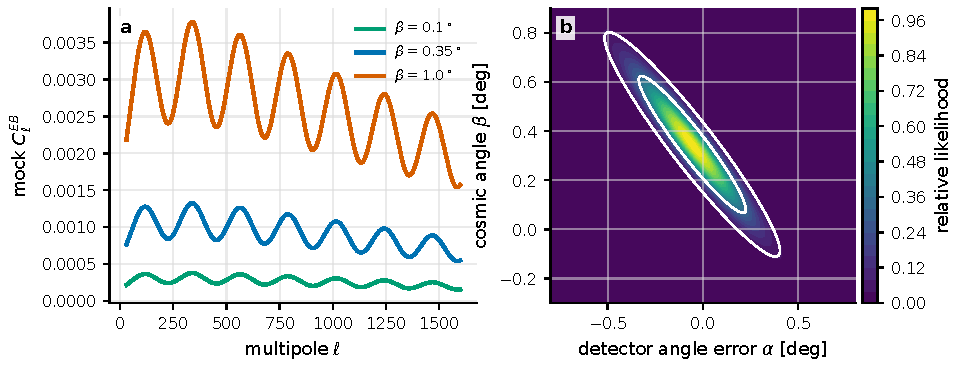
\includegraphics[width=0.94\linewidth]{figures/generated/chapter_15/ch15_cosmic_birefringence.pdf}
\caption{Cosmic birefringence 同时涉及 \(E/B\) 混合和仪器角标定。左图用 toy \(EE\) 与 \(BB\) 谱显示 \(\beta\) 如何产生 \(EB\)。右图显示 \(\alpha\) 与 \(\beta\) 的退化：若只看 CMB，探测器角误差和宇宙旋转几乎等价；利用前景频率依赖可以部分打破退化。}
\label{fig:ch15-cmb-birefringence}
\end{figure}

\Needspace{12\baselineskip}
单光子偏振事件表把这个问题从平均 map 推向时间域。一个偏振事件可写作
\begin{equation}
  e_q=(t_q,\nu_q,\hat{\bf n}_q,p_q,w_q),
  \label{eq:ch15-polarization-event}
\end{equation}
\begin{formulaexplain}[公式 (15.9) 解读]
\(e_q\) 是第 \(q\) 个偏振事件，包含时间、频率、方向、偏振通道和权重。把数据保留为事件表，可以在时间和频率维度上寻找共同旋转，而不必先平均成一张固定角度图。
\end{formulaexplain}
\(p_q\) 是偏振通道，\(w_q\) 是质量权重。若偏振角存在小的公共振荡，事件概率可以写成
\begin{equation}
  P(p_q|t_q,\nu_q,\hat{\bf n}_q)
  =
  P_0\!\left[p_q\,\middle|\,\psi_{\rm src}+\psi_{\rm prop}(\nu_q,\hat{\bf n}_q)+\delta\psi(t_q,\hat{\bf n}_q)\right].
  \label{eq:ch15-event-likelihood}
\end{equation}
\begin{formulaexplain}[公式 (15.10) 解读]
\(P_0\) 是给定总偏振角后的偏振通道概率，\(\psi_{\rm src}\) 是源本征项，\(\psi_{\rm prop}\) 是传播和仪器项，\(\delta\psi\) 是待检验的新物理旋转。这条式子把异常角度拆成可互相反驳的几类来源。
\end{formulaexplain}
\(\psi_{\rm src}\) 是源本征偏振，\(\psi_{\rm prop}\) 包括 Faraday、尘埃和仪器 Mueller 矩阵，\(\delta\psi\) 是要检验的新物理项。事件表可以在不同时间、频率和偏振通道之间做同一个似然，避免过早把数据平均成一个固定偏振角。代价也很直接：如果 Mueller 矩阵非对角项只知道到 \(10^{-3}\)，而目标旋转是 \(10^{-3}\,{\rm rad}\)，系统误差已经和信号同量级。强场 QED 真空双折射候选、孤立中子星光学偏振和 magnetar X-ray 偏振都要求先建模源几何和传播效应，偏振异常才可能被解释为新物理 \citep{2017MNRAS.465..492M}。

\section{脉冲星、FRB 和黑洞怎样提供前景检验}

CMB 给出全天平均的角度检验；脉冲星、FRB 和黑洞附近偏振则把问题推向时间域和强场环境。它们的优点是信号可以随时间、频率或黑洞尺度有特定模板；缺点是本征源结构和传播前景都很强。真正有用的策略，是把“共同时间项”“\(\lambda^2\) 前景”“黑洞质量标度”这些可区分特征放在同一个似然里。

脉冲星适合做时间域阵列，因为它们有稳定相位和重复脉冲。超轻标量暗物质的引力势振荡可在 PTA 中产生窄带 timing residual。若势扰动写成 \(\Psi_c\cos(2m_at+\varphi)\)，一个简化残差可写作
\begin{equation}
  R_\alpha(t)
  \simeq
  \frac{\Psi_c}{2\pi f}
  \left[
  \sin(2\pi ft+\varphi_E)
  -
  \sin(2\pi f(t-D_\alpha/c)+\varphi_\alpha)
  \right],
  \label{eq:ch15-pta-residual}
\end{equation}
\begin{formulaexplain}[公式 (15.11) 解读]
\(R_\alpha(t)\) 是第 \(\alpha\) 颗脉冲星的计时残差，\(\Psi_c\) 是势振荡幅度，\(f\) 是窄带频率。第一项是共同 Earth term，第二项是每颗脉冲星自己的 pulsar term。
\end{formulaexplain}
\(\alpha\) 标记第 \(\alpha\) 颗脉冲星，\(D_\alpha\) 是距离，\(f\simeq m_a/\pi\) 是势振荡频率。\(m_a\sim10^{-23}\,{\rm eV}\) 对应 \(f\sim10^{-8}\,{\rm Hz}\)，正好落在 PTA 的 \(10^{-9}-10^{-7}\,{\rm Hz}\) 窗口。Porayko 和 Postnov 对 NANOGrav 旧数据的分析给出 \(\Psi_c<1.14\times10^{-15}\) 的 95\% C.L. 上限，对应 \(f=1.75\times10^{-8}\,{\rm Hz}\) 处 \(h_c<4\times10^{-15}\) 的数量级 \citep{2014PhRvD..90f2008P}。在窄带随机背景近似中，不同脉冲星之间的相关可近似为
\begin{equation}
  \zeta_{\alpha\beta}=\frac{1}{2}(1+\delta_{\alpha\beta}),
  \label{eq:ch15-pta-correlation}
\end{equation}
\begin{formulaexplain}[公式 (15.12) 解读]
\(\zeta_{\alpha\beta}\) 是两颗脉冲星残差的相关系数，\(\delta_{\alpha\beta}\) 是 Kronecker delta。这个标量暗物质模板几乎不依赖两颗脉冲星的夹角，因此不同于张量引力波背景的 Hellings-Downs 曲线。
\end{formulaexplain}
这和随机引力波背景的 Hellings-Downs 角相关不同。若未来做“脉冲星偏振阵列”，同样要把共同 Earth term、本征磁层偏振、星际 Faraday 旋转、profile mode changes 和接收机偏振泄漏分开。

\begin{figure}[tbp]
\centering
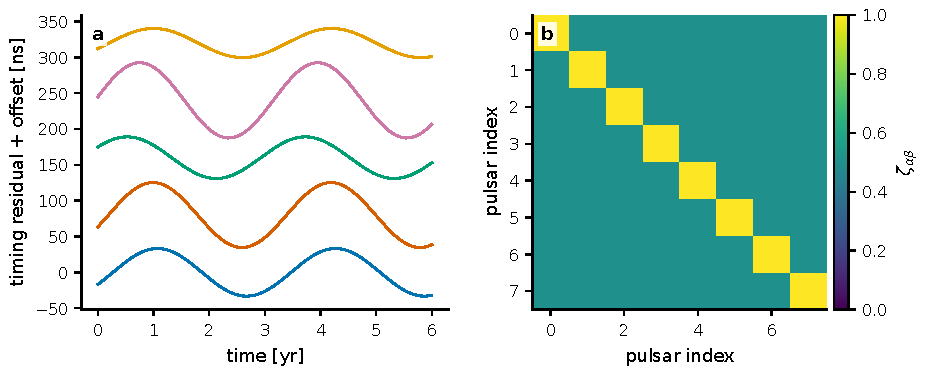
\includegraphics[width=0.94\linewidth]{figures/generated/chapter_15/ch15_pulsar_array_correlation.pdf}
\caption{脉冲星阵列里的共同窄带信号。左图是一个公共 Earth term 叠加每颗脉冲星自己的 pulsar term；曲线被人为错开以便观看。右图给出标量势振荡模型中的简化相关矩阵 \(\zeta_{\alpha\beta}=(1+\delta_{\alpha\beta})/2\)，它不同于随机张量引力波背景的角相关。}
\label{fig:ch15-pulsar-array}
\end{figure}

FRB 的偏振信息强，但传播前景也强。FRB 121102 在 \(z=0.193\) 的宿主星系中，4-8 GHz bursts 显示接近 \(100\%\) 线偏振，并有源框架 \({\rm RM}_{\rm src}=1.46\times10^5\) 和 \(1.33\times10^5\,{\rm rad\,m^{-2}}\) 的高而变化的 Faraday rotation measure；同一批 burst 还含有 \(\lesssim30\,\mu{\rm s}\) 的窄结构。若宿主贡献 \({\rm DM}_{\rm host}\sim70-270\,{\rm pc\,cm^{-3}}\)，对应的视线磁场下限为 mG 量级，远高于普通银河系 ISM 的 \(\sim5\,\mu{\rm G}\) \citep{2018Natur.553..182M}。这类源可作为极端磁化等离子体实验室；一个看似波长无关的偏振变化，仍要排除通道平均导致的 depolarization、RM 时间变化和 plasma lensing 选择效应。

\begin{figure}[tbp]
\centering
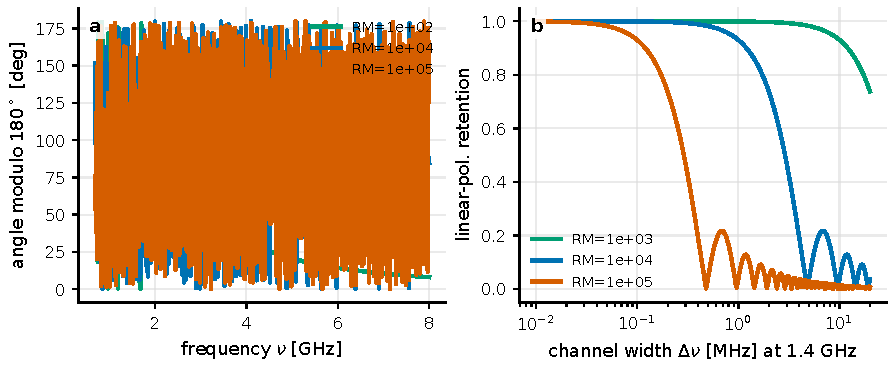
\includegraphics[width=0.94\linewidth]{figures/generated/chapter_15/ch15_frb_faraday_foreground.pdf}
\caption{FRB 偏振前景可以轻易淹没小旋转信号。左图显示不同 RM 下偏振角随频率的模 \(180^\circ\) 缠绕；\({\rm RM}=10^5\,{\rm rad\,m^{-2}}\) 在 GHz 频段变化极快。右图显示 \(1.4\,{\rm GHz}\) 附近有限通道宽度造成的线偏振保留率，窄通道是测高 RM 的必要条件。}
\label{fig:ch15-frb-faraday}
\end{figure}

\Needspace{11\baselineskip}
黑洞超辐射把轻玻色场和偏振图像连在一起。Kerr 黑洞角速度为 \(\Omega_H\)，玻色模满足
\begin{equation}
  \omega < m\Omega_H
  \label{eq:ch15-superradiance-condition}
\end{equation}
\begin{formulaexplain}[公式 (15.13) 解读]
\(\omega\) 是玻色模频率，\(m\) 是方位量子数，\(\Omega_H\) 是 Kerr 黑洞视界角速度。满足不等式时，波从黑洞自转中抽取能量，形成超辐射增长。
\end{formulaexplain}
时可从黑洞自转中抽取能量。定义
\begin{equation}
  \alpha_G=\frac{GM_\bullet m_a}{\hbar c},
  \label{eq:ch15-alpha-g}
\end{equation}
\begin{formulaexplain}[公式 (15.14) 解读]
\(\alpha_G\) 是黑洞引力半径和轴子 Compton 波长的比值，\(M_\bullet\) 是黑洞质量。它决定玻色云是否和黑洞尺度匹配；\(\alpha_G\sim0.1-1\) 时增长通常最有效。
\end{formulaexplain}
当 \(\alpha_G\sim0.1-1\) 时，玻色 Compton 波长与黑洞尺度匹配，云增长最快。相应轴子质量为
\begin{equation}
  m_a
  \simeq
  1.34\times10^{-10}\,{\rm eV}\,
  \alpha_G
  \left(\frac{M_\odot}{M_\bullet}\right).
  \label{eq:ch15-bh-mass-window}
\end{equation}
\begin{formulaexplain}[公式 (15.15) 解读]
这条式子把黑洞质量 \(M_\bullet\) 映射到最敏感的轴子质量 \(m_a\)。黑洞越重，对应的轴子质量窗口越低；因此 Sgr A* 和 M87* 探测的是不同超轻质量区。
\end{formulaexplain}
对 Sgr A* 的 \(4.3\times10^6M_\odot\)，\(\alpha_G=0.4\) 对应 \(m_a\simeq1.2\times10^{-17}\,{\rm eV}\)；对 M87* 的 \(6.5\times10^9M_\odot\)，对应 \(8\times10^{-21}\,{\rm eV}\)。EHT 偏振图像中的 axion cloud 模型预言，偏振角可随轴子周期振荡：Sgr A* 的周期可为 \(100-1000\,{\rm s}\)，M87* 可为数天，空间分辨率会决定这种振荡是否被环上不同方位平均掉 \citep{2015LNP...906.....B,2015CQGra..32m4001B,2017PhRvD..96c5019B,2020PhRvL.124f1102C,2022NatAs...6..592C}。

\begin{figure}[tbp]
\centering
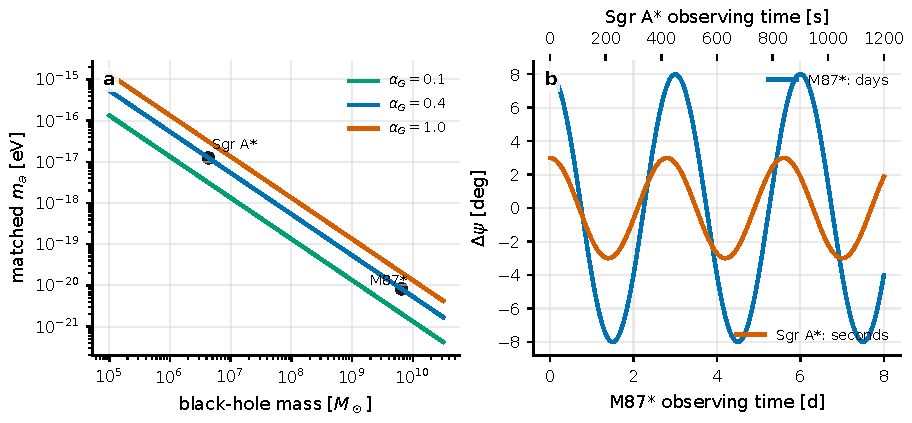
\includegraphics[width=0.94\linewidth]{figures/generated/chapter_15/ch15_black_hole_axion_cloud.pdf}
\caption{黑洞质量把超辐射轴子质量窗口定出来。左图用 \(\alpha_G=GM_\bullet m_a/\hbar c\) 标出不同黑洞质量对应的 \(m_a\)；Sgr A* 和 M87* 落在不同超轻质量区。右图画出 EHT 偏振角振荡的两个典型时间尺度：M87* 可在天尺度采样，Sgr A* 则需要秒到分钟级偏振成像。}
\label{fig:ch15-bh-axion}
\end{figure}

\section{暗物质小尺度透镜怎样把质量变成角偏移}

偏振检验寻找的是场对光子的量子通道影响；小尺度透镜检验寻找的是暗物质质量分布对光线路径的影响。两者共同点是信号常常不表现为“看到一团暗物质”，而表现为某个可观测量偏离普通模型。对透镜来说，这个可观测量可以是像位置、放大率、时间延迟或背景源的天体测量漂移。

暗物质存在本身可由星系团碰撞、弱透镜和动力学多种证据支持；Bullet Cluster 是经典例子，弱透镜质量峰与 X-ray 气体分离，表明主要质量成分近似无碰撞 \citep{2006ApJ...648L.109C,1993ApJ...404..441K}。小尺度结构给出另一类检验。CDM 数值模拟预言银河 halo 中有大量子晕和潮汐流，质量函数可延伸到远低于可见卫星星系的范围；Moore、Diemand 等结果使“暗的子结构”成为强透镜异常的重要候选解释 \citep{1994ApJ...427L...1F,1999ApJ...524L..19M,2008Natur.454..735D}。

子结构透镜的基本量级来自 Einstein 角
\begin{equation}
  \theta_E
  =
  \left(
  \frac{4GM}{c^2}
  \frac{D_{ls}}{D_lD_s}
  \right)^{1/2}.
  \label{eq:ch15-subhalo-einstein}
\end{equation}
\begin{formulaexplain}[公式 (15.16) 解读]
\(\theta_E\) 是子晕 Einstein 角，\(M\) 是透镜质量，距离组合给出几何效率。质量越大，角尺度按 \(M^{1/2}\) 增长；这直接决定强透镜异常需要的角分辨率。
\end{formulaexplain}
对 \(D_l\simeq1\,{\rm Gpc}\)、\(D_s\simeq2\,{\rm Gpc}\) 的星系强透镜，\(10^8M_\odot\) 子晕的 \(\theta_E\) 是几十 mas 量级，\(10^6M_\odot\) 则是几 mas。若像与子晕角距离为 \(b\gg\theta_E\)，点质量近似的天体测量偏移量为
\begin{equation}
  \delta\theta\simeq\frac{\theta_E^2}{b}.
  \label{eq:ch15-astrometric-shift}
\end{equation}
\begin{formulaexplain}[公式 (15.17) 解读]
\(\delta\theta\) 是天体测量偏移，\(b\) 是像到子晕的角距离。子晕越接近像、\(\theta_E\) 越大，位置扰动越明显；远离时信号按 \(1/b\) 变小。
\end{formulaexplain}
这个数量级把分辨率要求摆得很清楚：\(10^6M_\odot\) 子晕在 \(b=10\,{\rm mas}\) 处只给 \(\mu{\rm as}\) 量级偏移。强透镜 flux-ratio anomalies 对放大率扰动敏感，Mao 与 Schneider 指出低质量子结构可解释一些四像系统的异常；Dalal 与 Kochanek 用 7 个 radio lens 得到子结构质量分数中位数 \(f_{\rm sat}\simeq0.02\)，90\% 范围约 \(0.006-0.07\)；Vegetti 和 Hezaveh 等用 gravitational imaging 和 ALMA 数据把单个暗子结构探测推进到空间分辨建模 \citep{1998MNRAS.295..587M,2002ApJ...572...25D,2010MNRAS.408.1969V,2016ApJ...823...37H}。

\begin{figure}[tbp]
\centering
\includegraphics[width=0.94\linewidth]{figures/generated/chapter_15/ch15_dark_matter_lensing.pdf}
\caption{暗物质子晕的透镜信号受角尺度限制。左图给出典型 Gpc 几何下子晕 Einstein 角随质量的变化。右图把 \(\delta\theta\simeq\theta_E^2/b\) 转换为天体测量偏移；低质量子晕需要 mas 级接近和 \(\mu{\rm as}\) 级系统控制才容易看见。}
\label{fig:ch15-dm-lensing}
\end{figure}

Gaia 和未来天体测量巡天把这个问题变成时间域：子晕横穿背景源附近时，位置偏移随时间变化。若子晕横向速度 \(v_\perp\sim200\,{\rm km\,s^{-1}}\)，在 kpc 距离上对应 mas/yr 量级角速度；信号形状由 impact parameter、质量剖面和源自身 proper motion 共同决定。Mondino 等用 Gaia DR3 和未来 catalogues 讨论了这种 astrometric weak lensing 搜索，主要限制来自扫描定律、源密度、proper-motion covariance 和太阳系/仪器系统误差 \citep{2024MNRAS.531..632M}。PBH 暗物质也可通过透镜和动力学被限制，但质量函数、聚团和天体物理前景会改变解释 \citep{2016PhRvD..94h3504C}。

\section{怎样把异常写成可反驳的检验}

到这里为止，所有候选信号都有一个共同教训：异常本身不是结论，异常的可反驳结构才是结论。新物理搜索的观测量通常不止一个：偏振角、到达时间、像位置和放大率可能来自不同仪器，也有不同的统计误差和系统误差。把这些量合并为数据向量 \({\bf d}\) 后，模型可以分成
\begin{equation}
  {\bf m}({\boldsymbol\theta})
  =
  {\bf m}_{\rm src}
  +{\bf m}_{\rm prop}
  +{\bf m}_{\rm inst}
  +{\bf m}_{\rm new}({\boldsymbol\theta}),
  \label{eq:ch15-model-vector}
\end{equation}
\begin{formulaexplain}[公式 (15.18) 解读]
\({\bf m}\) 是模型预测向量，被拆成源、传播、仪器和新物理四项。这样的拆分强迫我们把异常先和普通天体物理、传播前景、校准误差放在同一个账本里比较。
\end{formulaexplain}
其中 \({\boldsymbol\theta}\) 包含 \(g_{a\gamma}\)、\(m_a\)、\(\beta\)、子晕质量函数或 PBH fraction 等参数。高斯近似下
\begin{equation}
  -2\ln\mathcal L
  =
  \left[{\bf d}-{\bf m}({\boldsymbol\theta})\right]^{\mathsf T}
  \left(C_{\rm stat}+C_{\rm sys}\right)^{-1}
  \left[{\bf d}-{\bf m}({\boldsymbol\theta})\right]
  +\ln\det(C_{\rm stat}+C_{\rm sys}).
  \label{eq:ch15-systematics-likelihood}
\end{equation}
\begin{formulaexplain}[公式 (15.19) 解读]
\(\mathcal L\) 是高斯似然，\(C_{\rm stat}\) 是统计协方差，\(C_{\rm sys}\) 是系统误差协方差。残差必须用两类误差共同加权；若漏掉系统项，单个异常会被错误地放大。
\end{formulaexplain}
\(C_{\rm stat}\) 来自 photon noise、TOA uncertainties 或图像噪声；\(C_{\rm sys}\) 包含 Mueller 矩阵、绝对偏振角、Faraday 前景、尘埃 EB、透镜宏模型、源结构和选择函数。若 \(C_{\rm sys}\) 未进入似然，单个异常点会被过度解释。

这些信号有清楚的相互区分方式。Faraday 旋转随 \(\lambda^2\) 变，轴子背景旋转近似 achromatic；静态 cosmic birefringence 在 CMB 中产生全局 EB/TB，超轻暗物质会在观测时间上振荡；黑洞轴子云应与黑洞质量、spin、环上方位和观测时间相关；暗物质子晕透镜应同时扰动像位置、放大率和时间延迟，而恒星表面结构主要随源旋转、波长和基线方向变化。可信结果通常要经受样本统计、空场或控制源、频率反演、时间相干性和仪器重标定的交叉检查。

CMB 和早期宇宙涨落把同一要求推到全天图层面。那里的观测对象不再是单个源的偏振角或透镜像，而是 \(T/E/B\) 图、功率谱、偏振角和系统误差矩阵。

